\documentclass[norsk,a4paper,11pt]{article}
\usepackage[T1]{fontenc} %for å bruke æøå
\usepackage[utf8]{inputenc}
\usepackage{graphicx} %for å inkludere grafikk
\usepackage{verbatim} %for å inkludere filer med tegn LaTeX ikke liker
\usepackage{mathpazo}
\usepackage{listings}
\bibliographystyle{plain}
\usepackage{xcolor}
\usepackage{float}
\usepackage{amsmath}
\usepackage{hyperref}



\setlength{\parindent}{0em}

\definecolor{background}{gray}{0.9}
\definecolor{comment}{rgb}{0.6,0.4,0.8}
\definecolor{string}{rgb}{0.6,0.4,0.8}
\definecolor{keyword}{rgb}{0.9,0.17,0.31}
\lstset{
	title=\lstname,
	numberstyle=\tiny, 
	breaklines=true,
	tabsize=4,
	language=Python,
	morekeywords={with,super,as},,
	frame=single,
	basicstyle=\footnotesize\tt,
	commentstyle=\color{comment},
	keywordstyle=\color{keyword},
	stringstyle=\color{string},
	backgroundcolor=\color{background},
	showstringspaces=false,
	numbers=none,
	numbersep=5pt,
	literate=
		{æ}{{\ae}}1
		{å}{{\aa}}1
		{ø}{{\o}}1
		{Æ}{{\AE}}1
		{Å}{{\AA}}1
		{Ø}{{\O}}1
	}


\title{Project Fys3600}
\author{Candidate numbers: 1. \& 14.}
\date{\today}
\begin{document}

\maketitle

\begin{figure}[H]
	\begin{center}
		
\includegraphics[scale=1.0]{Figures/uiosegl.png}
	\end{center}
\end{figure}



\newpage

\tableofcontents

\section{Introduction} % (Introduction to project and theoretical background)
\label{sec:intro}
	As society moves towards more automatization, accurate, globally available navigational tools are coming in demand. A solution to this is using satellites. 			There are some problems however. Satellites (and in some cases even earthbound equipment) are susceptible to bad space weather. Having your self-			driving car suddenly acting up is not desirable. Predicting when equipment will be in danger of getting hit by high energy particles is therefore of interest.\\ 
	\\
	In this report, we will be looking at data from several instruments measuring properties of the solar wind and the interplanetary magnetic field (IMF) along 			with auroras and some ionospheric currents from 06.01.2011. We will also be looking at some potential consequences of the measurements.




\newpage
\subsection{Theory} % (The theoretical part of the intro)
\label{sub:theory}
	\subsubsection{The Sun:} 
		The root of all our problems is the star in the center of our solar system: the sun.\\
		\\
		\textbf{IMF}\\
		The sun, like the earth, has a magnetic field. This magnetic field stretches throughout the solar system, and has fittingly been dubbed the 						interplanetary magnetic field. What causes this magnetic field is beyond the scope of this report, but it is seemingly quite erratic, changing 				sign and field strength often.\\
		Something more constant about the imf is the general direction of the field lines. Due to the rotation of the sun, the magnetic field lines end up looking 			like archimedian spirals (or a ballerina skirt in 3 dimensions).
		\begin{figure}[H]
			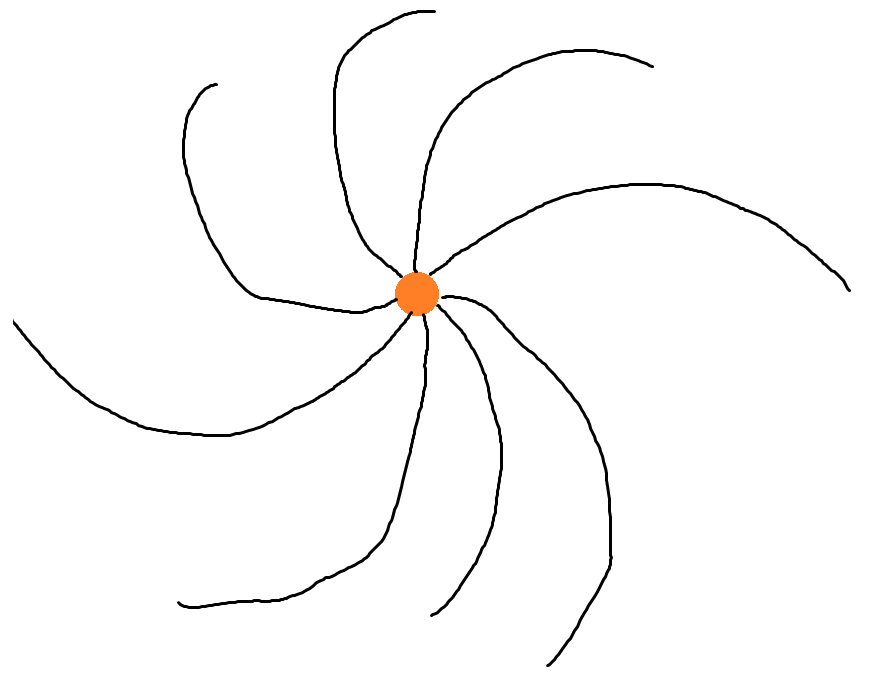
\includegraphics[scale = 0.3]{Figures/artistic_imf.png}
			\centering
			\caption{An artistic rendition of the interplanetary magnetic field. With the sun in the middle and rotating, the magnetic field lines end up forming 					     archimedian spirals.}
			\label{fig::spirals}
		\end{figure}

		\textbf{Solar Wind}\\
		Accompanying the magnetic field lines is plasma streams. Ejected from the suns corona, these plasma streams of varying velocity and density can also                         		be drawn like figure \ref{fig::spirals}.\\
		Carrying large amount of highly energized ionized particles, the solar wind is of great interest to us. Knowing the density and velocity of the solar wind 				is necesarry in understanding the consequences of its interactions with earth and its satellites.\\
		\\
		\textbf{Coronal mass ejection and solar flares}\\
		There are events where the sun sends out relatively huge amounts of plasma and radiation.\\
		One such event is a solar flare. A solar flare is a massive outburst of radiation happening in the lower corona. Being composed of mostly photons, a 				solar flare does not follow the magnetic field lines.\\
		Another such event is a coronal mass ejection (CME). During times of magnetic unrest, the sun might eject massive amounts of mass from its corona. 				Such outbursts are sometimes several times larger than the sun in diameter. The mass ejected follows the magnetic field lines, and ends up causing a 		spike in the solar wind density, something that can be harmful to instruments on earth.
		\begin{figure}[H]
			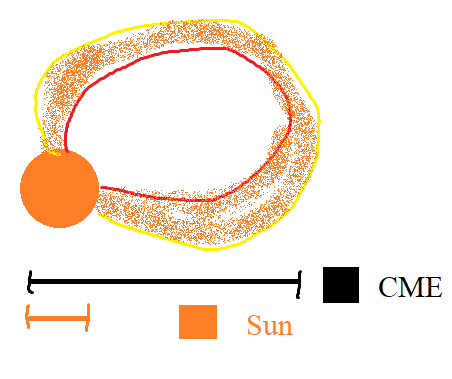
\includegraphics[scale = 0.7]{Figures/artistic_cme.png}
			\centering
			\caption{Artistic size comparison between the sun and a possible cme. As one can see, the cme can be many times larger in size than the sun.}
			\label{fig::cme}
		\end{figure}

\newpage
	\subsubsection{The Magnetosphere:}
		Like the sun, the earth also has a magnetic field.
		\begin{figure}[H]
			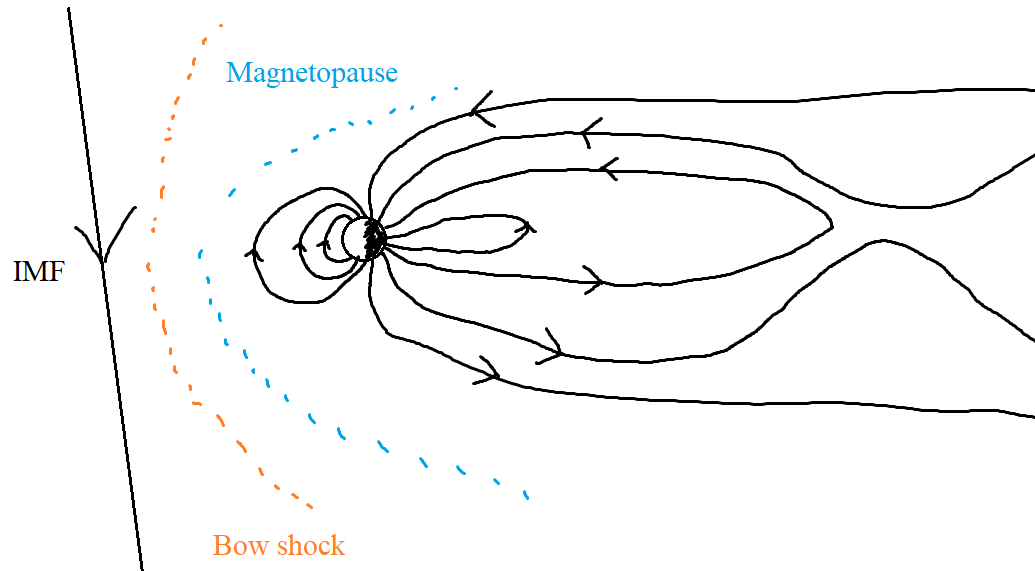
\includegraphics[scale = 0.5]{Figures/magnetosphere.png}
			\centering
			\caption{The earths magnetosphere. Note that it looks a bit different when the IMF Z component has the same sign as earths (in the figure, they 						     are opposite).}
			\label{fig::magnetopause}
		\end{figure}
	
	The earths magnetic south pole is currently located on the north pole. This means that the magnetic field goes from the geographical south pole to the 			geographical north pole. In figure \ref{fig::magnetopause}, this is indicated by arrows pointing along the field lines.

	\textbf{Magnetic reconnection}\\
	We observe many magnetosphere-related events from earth, such as the aurora. As these are not happening all the time, something must happen to 				trigger them.\\  
	When the Z (north/south) direction of the IMF and earths magnetic field points in opposite directions, field lines from earth and field lines from the IMF can 			break and recouple with eachother. This phenomenon is known as magnetic reconnection.\\
	When magnetic reconnection happens, the field lines "wrap around the earth" in an attempt to regain equilibrium. We can divide this process into different 			stages of what we call the Dungey cycle.
	\begin{figure}[H]
		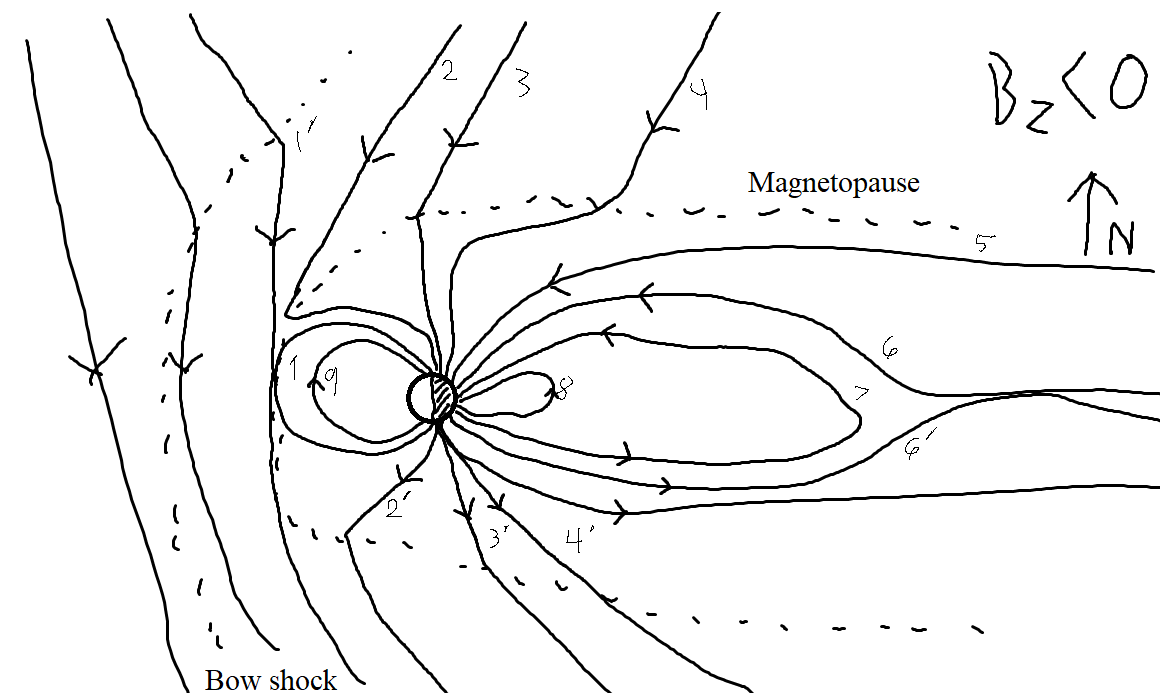
\includegraphics[scale = 0.5]{Figures/Dungey_cycle_negative.png}
		\centering
		\caption{A figure explaining the Dungey cycle. The numbers indicate the stages of the cycle. The field lines start off with a reconnection on the day-						side, then proceeds to wrap around to the night side. We then get another reconnection at 6, and the field lines settle down. }
		\label{fig::dungey_cycle}
	\end{figure}

	\subsubsection{Ionospheric currents}
	The Dungey cycle is important, as magnetic reconnection is the main perpetrator in accelerating plasma into the polar cusps.\\
	There are several plasma currents in the ionosphere ($\approx$ 75-1000km above sea level).
	\begin{figure}[H]
		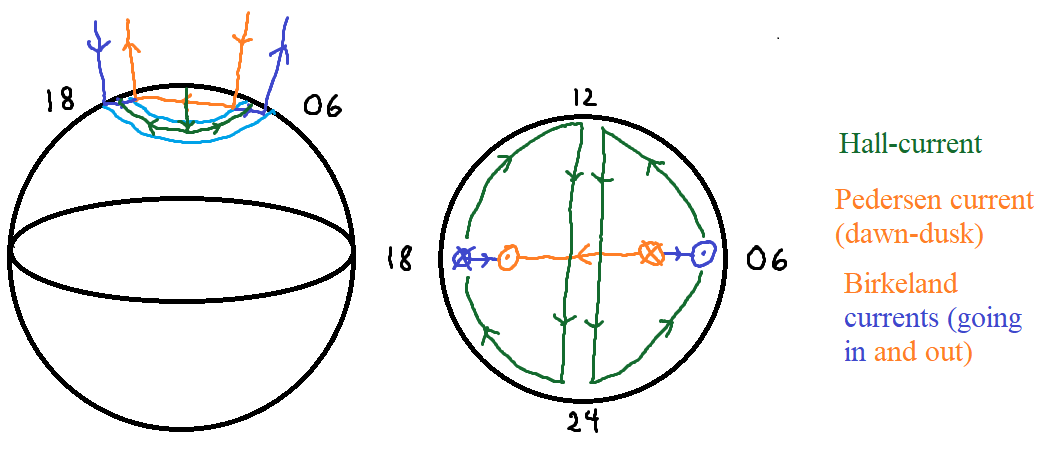
\includegraphics[scale = 0.7]{Figures/ionosphere_currents.png}
		\centering
		\caption{Some ionospheric currents. Here we see the Birkeland currents stretching out from the polar cusp, the Pedersen current going from dawn to 						dusk and Hall-currents going from day to night, and back around the cusp. The numbers indicate magnetic local time, with 12 being dayside 			and 06 being dawn.}

		\label{fig::ionosphere}
	\end{figure}
	One of these is the Birkeland currents which bring plasma in and out of the polar cusps. The cause of this is the interaction between the magnetosphere and 	the IMF.\\
	As the charged particles in the Birkeland currents approach earth, their density increases. This increases their collisions rate, which in turn causes the ions 			and electrons to drift apart (since they gyrate in opposite directions). This causes another current in the lower ionosphere: the Pedersen current (the orange 	and purple lines 	going along the earth in figure \ref{fig::ionosphere}).\\
	Since the Pedersen current includes a divition in charge, we also end up with an E field. This, along with the B field lines that point towards the polar cusp 			introduces another current through E $\times$ B drift: the Hall-current which is depicted in green in figure \ref{fig::ionosphere}.\\
	Along with these current systems, we can also observe 630 nm (red) and 557 nm (green) light from the lower ionosphere as charged particles hit and 			excite oxygen. This is the phenomenon known as aurora borealis; the northern lights.\\
	\\
	Since all these phenomenon are caused by interactions in the magnetosphere, we can use them to say something about the IMF and the other way around. 
	


% subsection theory (end)

% section introduction (end)


\section{instruments} % (description of the instrumenst used in this project)
\label{sec:instruments}

\subsection{Ground based magnetometer; IMAGE}
Knowing the B field at ground level is of interest. Luckily for us, there is a network of groundbased magnetometers known as the International Monitor for Auroral Geomagnetic Effects; IMAGE.\\
\begin{figure}[H]
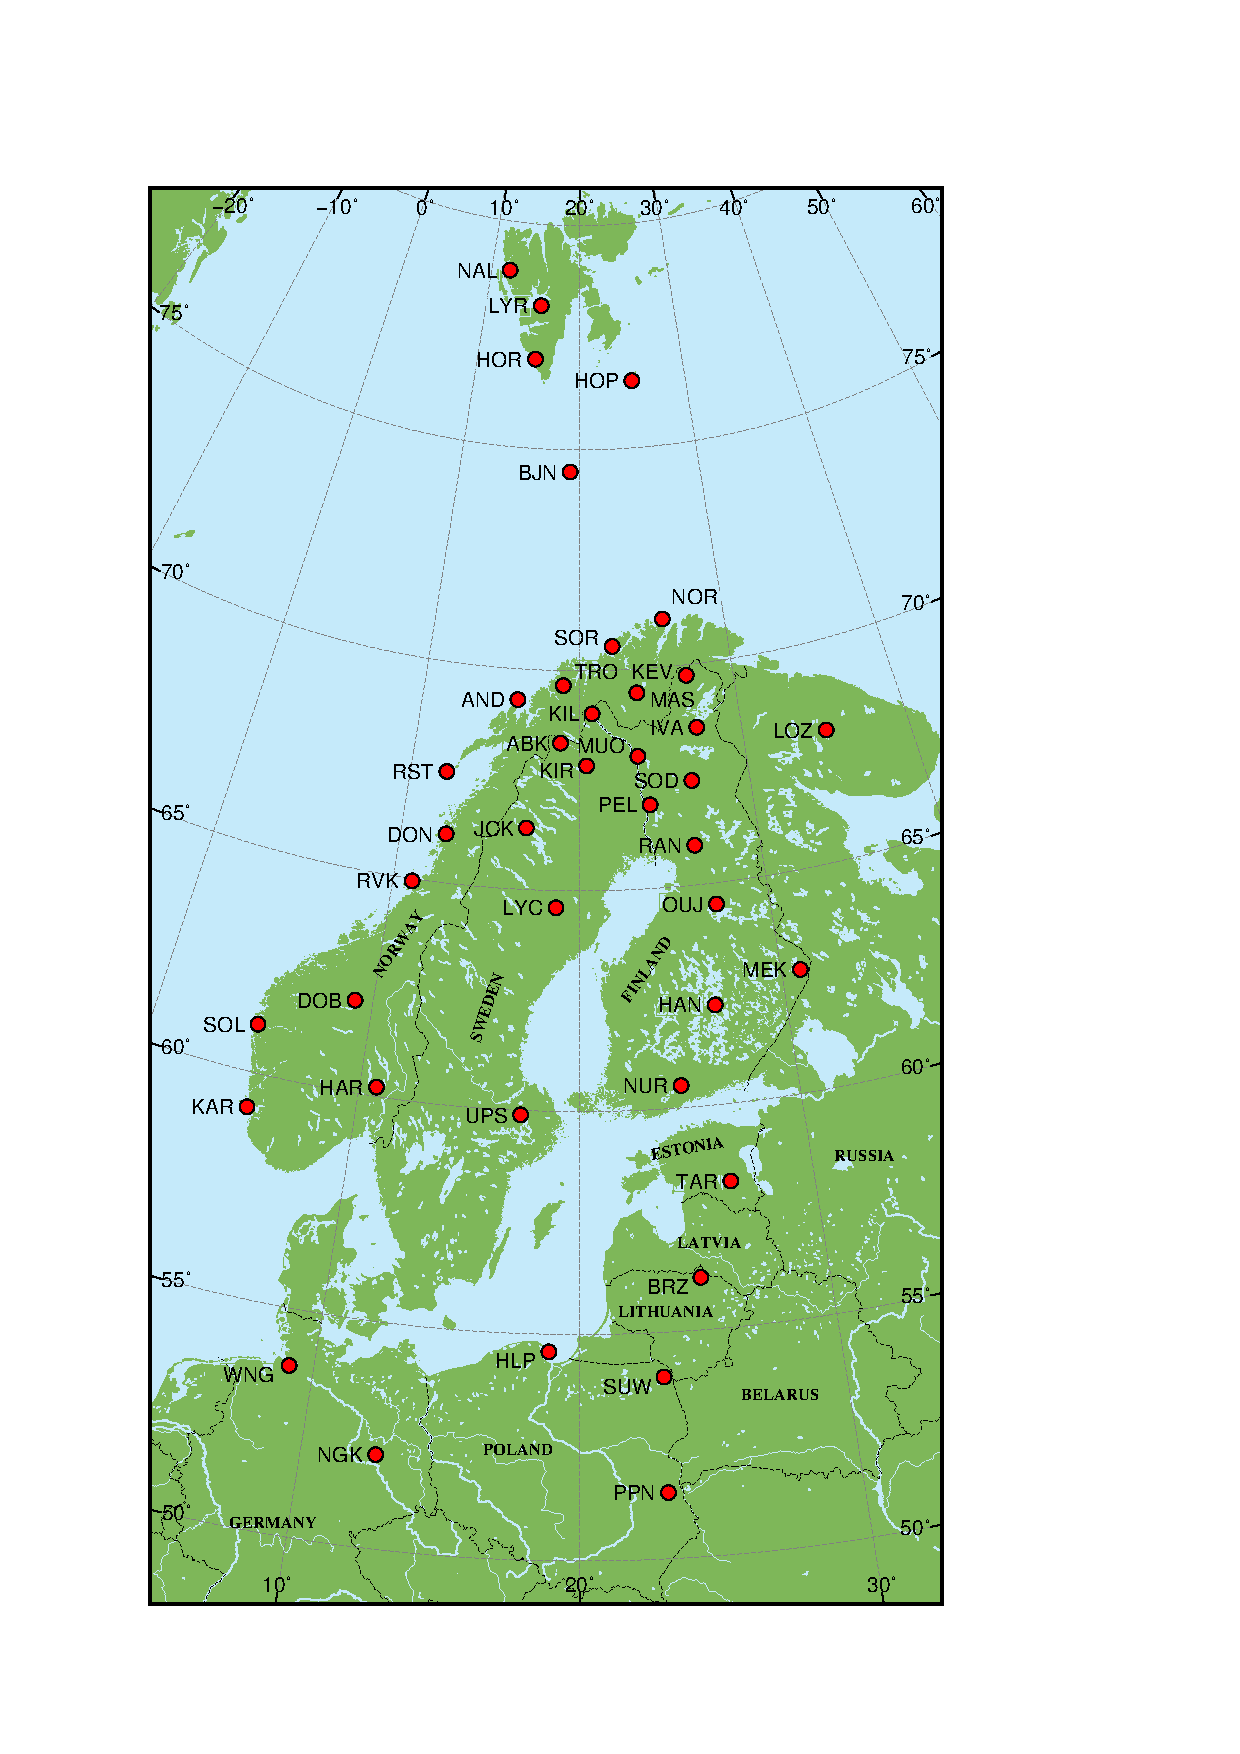
\includegraphics[scale = 0.5]{Figures/magnetometer_map.pdf}
\centering
\caption{A map showing the IMAGE stations. Source: http://space.fmi.fi/image/www/index.php?page=maps}
\label{fig::image_map}
\end{figure}

When charged particles start flowing in the ionosphere, it creates a B field in accordance with Ampere's law. For example, if we have a dawn-dusk current inside the polar circle, we can notice it by measuring the B field perpendicular to it.\\
Knowing the coordinate system used by IMAGE is important when reading its data. IMAGE operates using 3 coordinates: X, Y and Z.\\
The X coordinate always points towards the north pole from the magnetometer, akin to latitude. The Y coordinate always points towards the east, aking to longitude. The Z coordinate points towards the sky, perpendicular to the earth from where the magnetometer is.

\subsection{Super Dual Auroral Radar Network; SuperDARN}
SuperDARN is a network of radars used to measure plasma flow in the ionosphere. By using data from SuperDARN, one can make a convection flow chart that tells us what the Hall-current looks like at a certain time.

\subsection{All-Sky Camera}
As the auroras emit very specific wavelengths, it is possible to measure the level of auroras by measuring the intensity of these wavelengths. On Svalbard, the University of Oslo have placed All-Sky Imagers that measure the intensity of these wavelengths for much of the night sky by using a fish-eye lense, filters and a photon counter. By slicing these circular pictures into lines going from low to high latitude and combining them, one can make a keogram that describes the development of the aurora over time.\\
One must be careful when reading keograms however, as they are prone to errors due to atmospheric conditions. For example, if there are clouds, they will block a lot of the light. Clouds tend to drift across the sky, so its possible to tell from a glance that a keogram has been affected by clouds if the light from the auroras also seem to drift.

\subsection{Advanced Composition Explorer (ACE)} % (Short description of the ACE satellite)
\label{sub:ACE}
	In this project we are using data from a heliospheric satellite called ACE, which stands for Advanced Composition Explorer. ACE is a NASA satellite that gives us info about the solar wind. It is positioned in the L1 liberation point, about 1.5 million km from the Earth. The instrumentation on the satellite includes an Electron, Proton and Alpha Monitor(EPAM) from Johns Hopkins University Applied Physics Laboratory. Magnetic Field (MAG) from the University of Delaware Bartol Research Institute and subsequently University of New Hampshire. Solar Isotope Spectrometer (SIS) California Institute of Technology. Solar Wind Electron Proton and Alpha Monitor (SWEPAM) Los Alamos National Laboratory. We will be using the MAG and the SEWPAM. \\

	The MAG can give us the B-field magnitude and the magnetic field vector in different coordinate systems, such as GSM, GSE and RTN. The SWEPAM gives us information about the solar wind(SW) proton number density, the SW bulk speed, alpha to proton density ratio, the SW velocity in the same coordinate systems as the MAG and also the position of ACE.
% subsection ACE (end)

\subsection{Indices} % (Short description of the instrument indices)
\label{sub:indices}

\subsubsection{Dst (Disturbance storm time)} % (Dst explaind)
\label{sub:Dst}
With the Dst we can observe geomagnetic storms. The Dst is a quantification of the ring current and is an hourly scaling of the horizontal magnetic variation. Since the current flows in the equatorial magnetosphere, it is best sensed at low-latitude stations. These stations are sufficciently far from the equatorial electrojet so it is not disturbed by those ionospheric currents have litte effect on the magnetic field variations. The auroral currents also have little effect. They use the quiet days to establish the benchmark or background levels of the magnetic field and the average minimum ring current. This is then subtracted from the records so the disturbance is the important part. The world average is called the Dst. 
% subsubsection Dst (end)

\subsubsection{Auroral Electrojet (AE) Index} % (AE explained)
\label{sub:AE_index}
Using the AE index we can observe substorms. The AE index measures the strenght of the auroral current systems. These current are at low altitudes(near 100 km) and high latitudes (near 70$^\circ$). There are 12 stations that measure this. The AE is comprised of AU(upper envelope, eastward auroral electrojet) and AL(lower envelope, westward auroral electrojet), so AE = AU-AL which gives us the overall activity of the electrojets
% subsubsection AE index (end)

\subsubsection{Kp index} % (fold)
\label{sub:Kp_index}
I'l write about the KP index a little later
% subsection Kp index (end)

% subsection indices (end)




% section instruments (end)

\section{Observations} % (Detailed description of our observations, with all the graphs and figures nescessary)
\label{sec:observations}

\subsection{IMAGE data}
Here is the IMAGE data from the sixth of january 2011. As we can see, things are relatively quiet until around 10 pm. 
\begin{figure}[H]
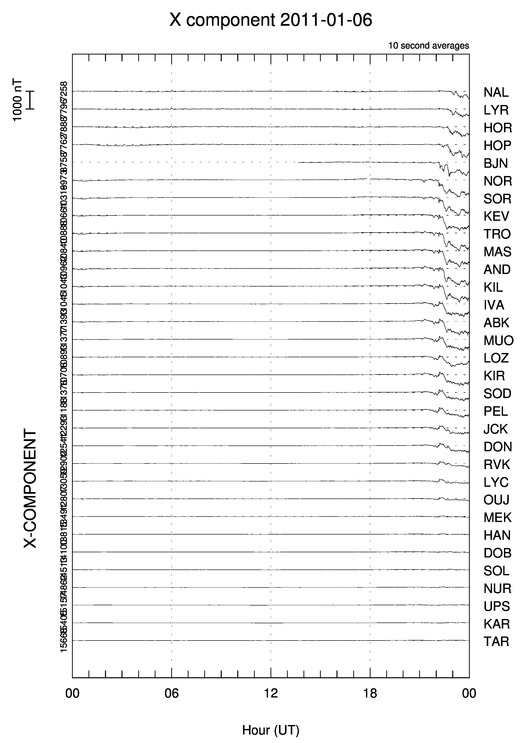
\includegraphics[scale = 0.9]{Figures/X_gram.jpg}
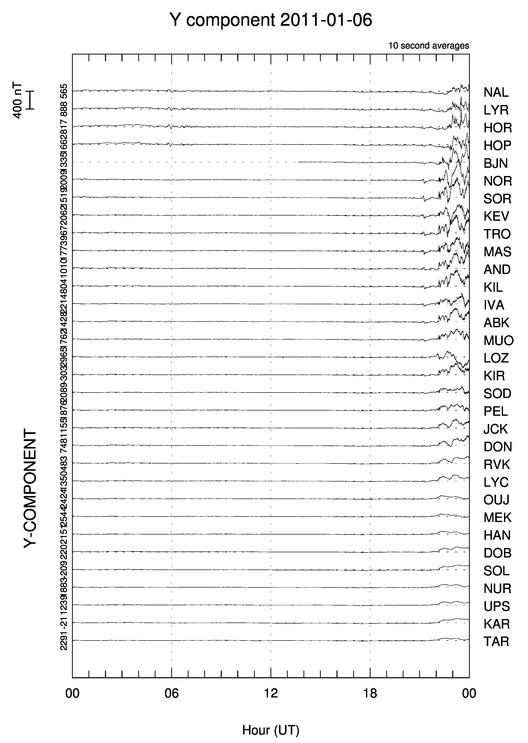
\includegraphics[scale = 0.9]{Figures/Y_gram.jpg}
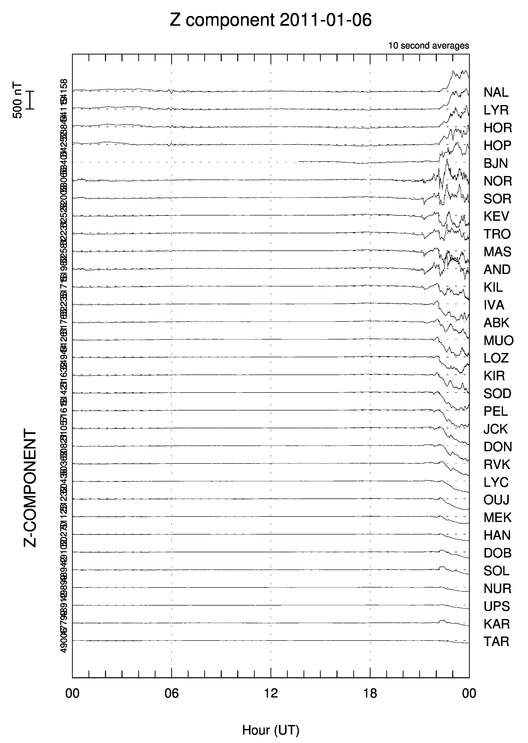
\includegraphics[scale = 0.9]{Figures/Z_gram.jpg}
\centering
\caption{IMAGE data. The letters on the side refer to stations seen in figure \ref{fig::image_map}. Source: http://space.fmi.fi/image/www/index.php?page=home }
\label{fig::image_data}
\end{figure}

\subsection{SuperDARN data}
Here is some of the data from SuperDARN for the sixth of january 2011. We have chosen to include data for times that indicate the development of the ionospheric currents over time. 

\begin{figure}[H]
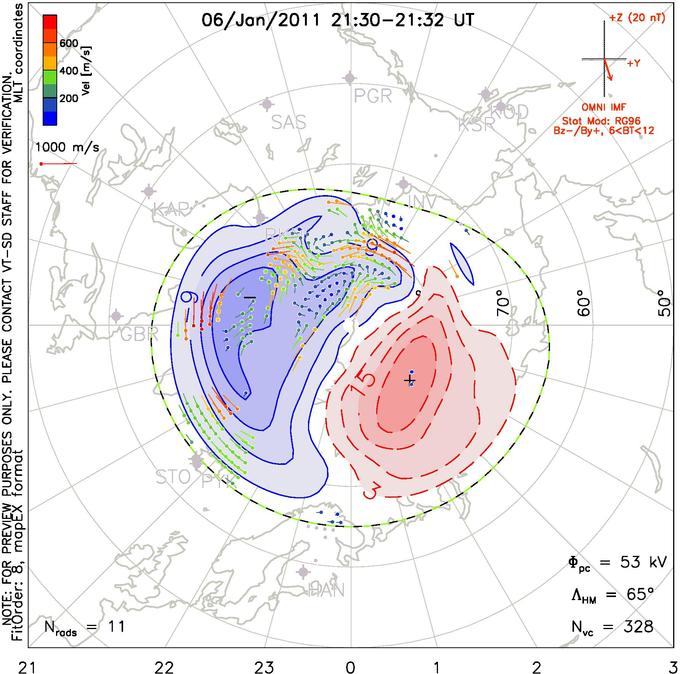
\includegraphics[scale = 1.0]{Figures/Superdarn/superdarn_21_30.jpg}
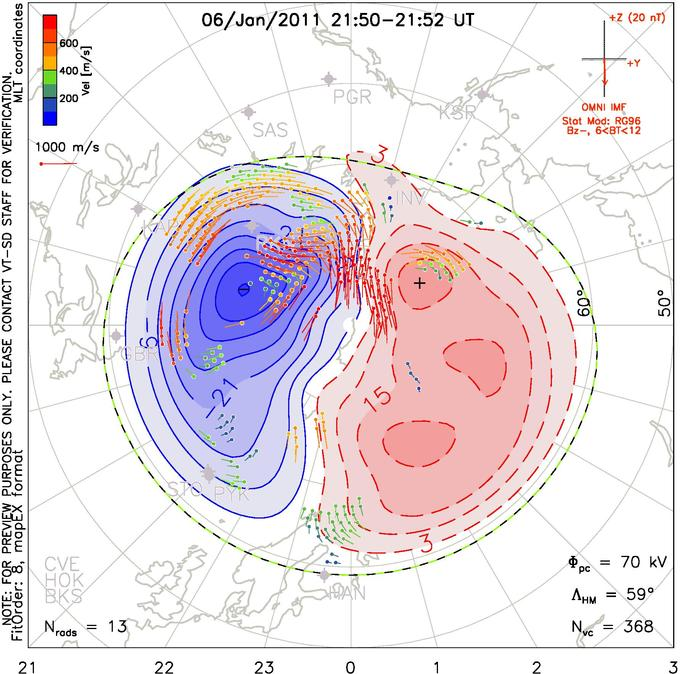
\includegraphics[scale = 1.0]{Figures/Superdarn/superdarn_21_52.jpg}
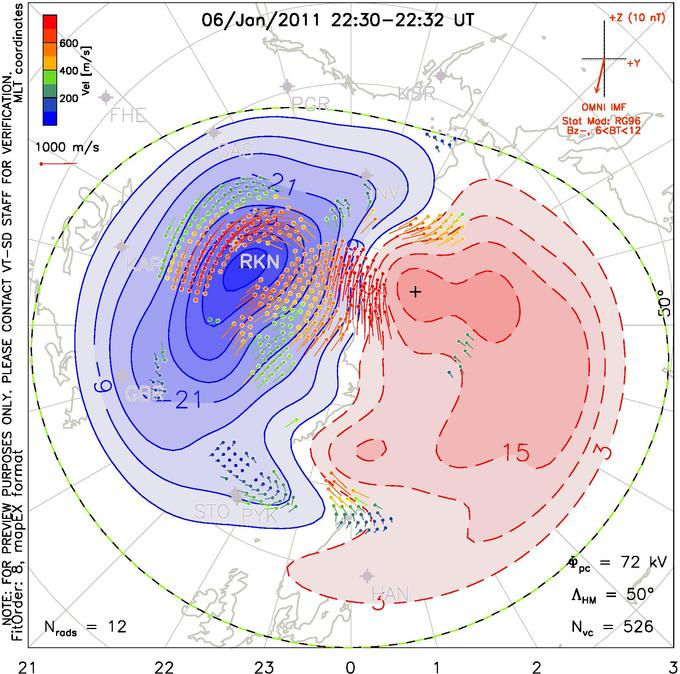
\includegraphics[scale = 1.0]{Figures/Superdarn/superdarn_22_32.jpg}
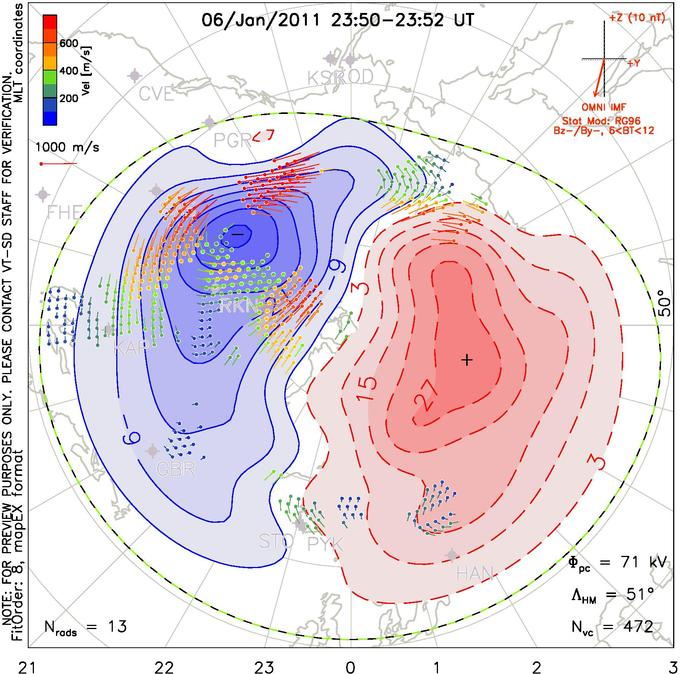
\includegraphics[scale = 1.0]{Figures/Superdarn/superdarn_23_52.jpg}
\centering
\caption{Convection maps derived from SuperDARN data. The vector arrows indicate measured data, while the streamlines indicate derived plasma flow. Source: http://vt.superdarn.org/tiki-index.php}
\label{fig::superdarn_data}
\end{figure}

\subsection{All-sky Camera data}
Here we have 2 keograms from the sixth of january 2011. The 2 keograms depict the development of auroras over time by measuring the intensity of 557 nm and 630 nm light.

\begin{figure}[H]
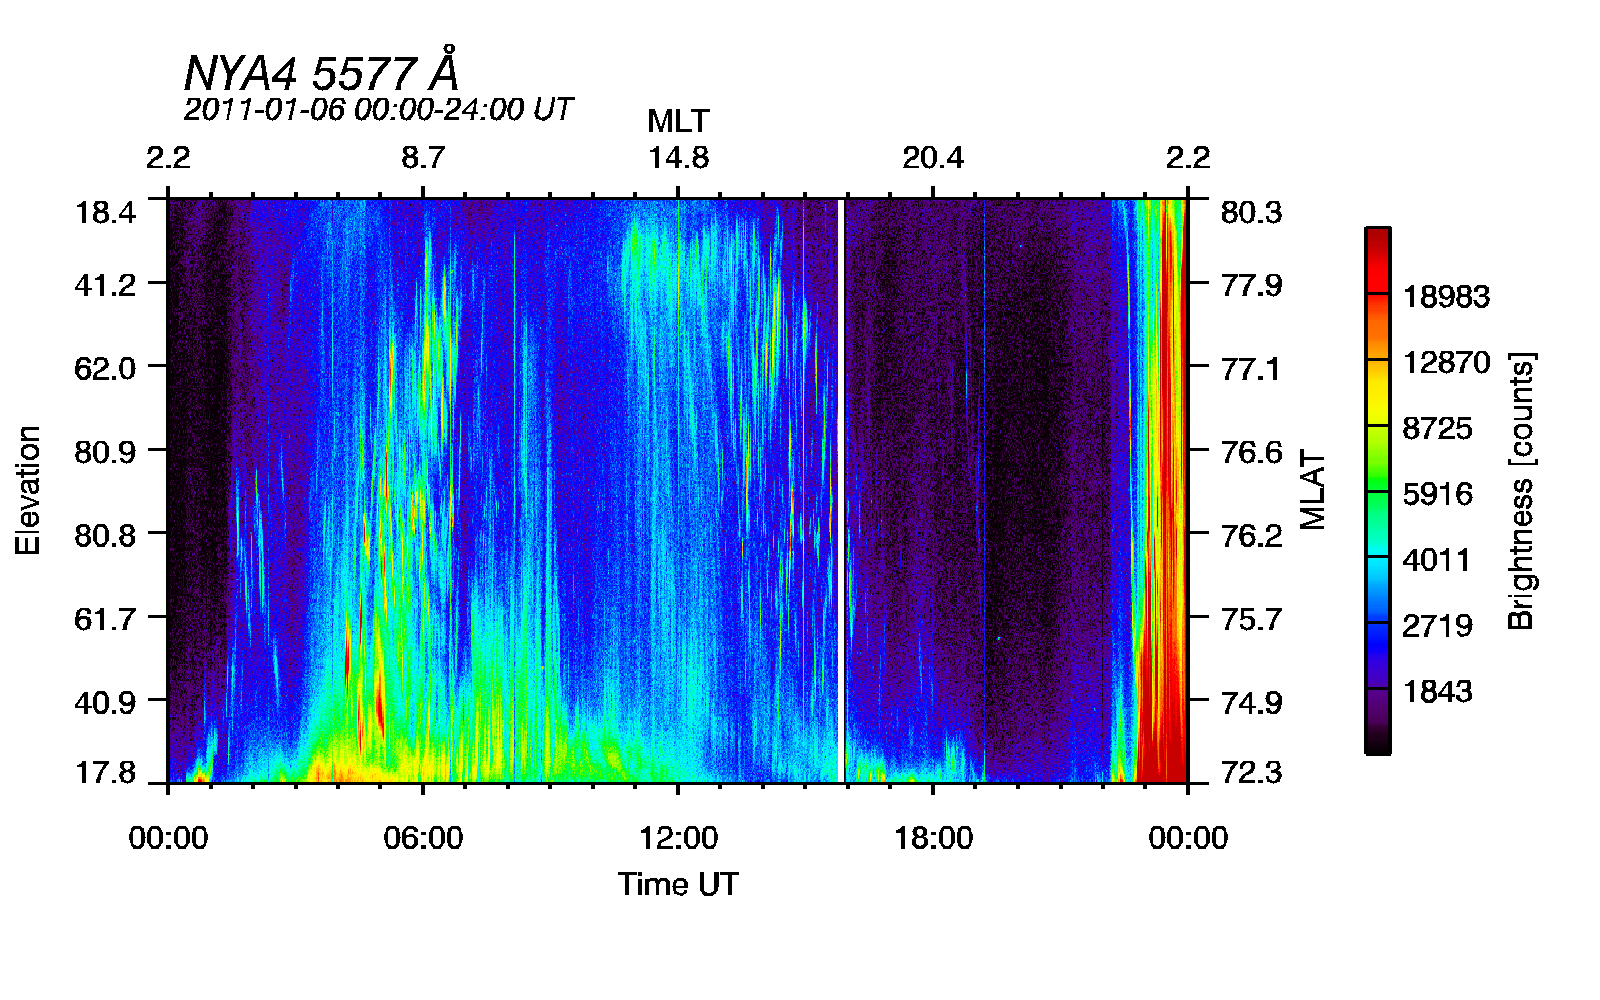
\includegraphics[scale = 0.2]{Figures/nya4_20110106_0000-2400_5577.png}
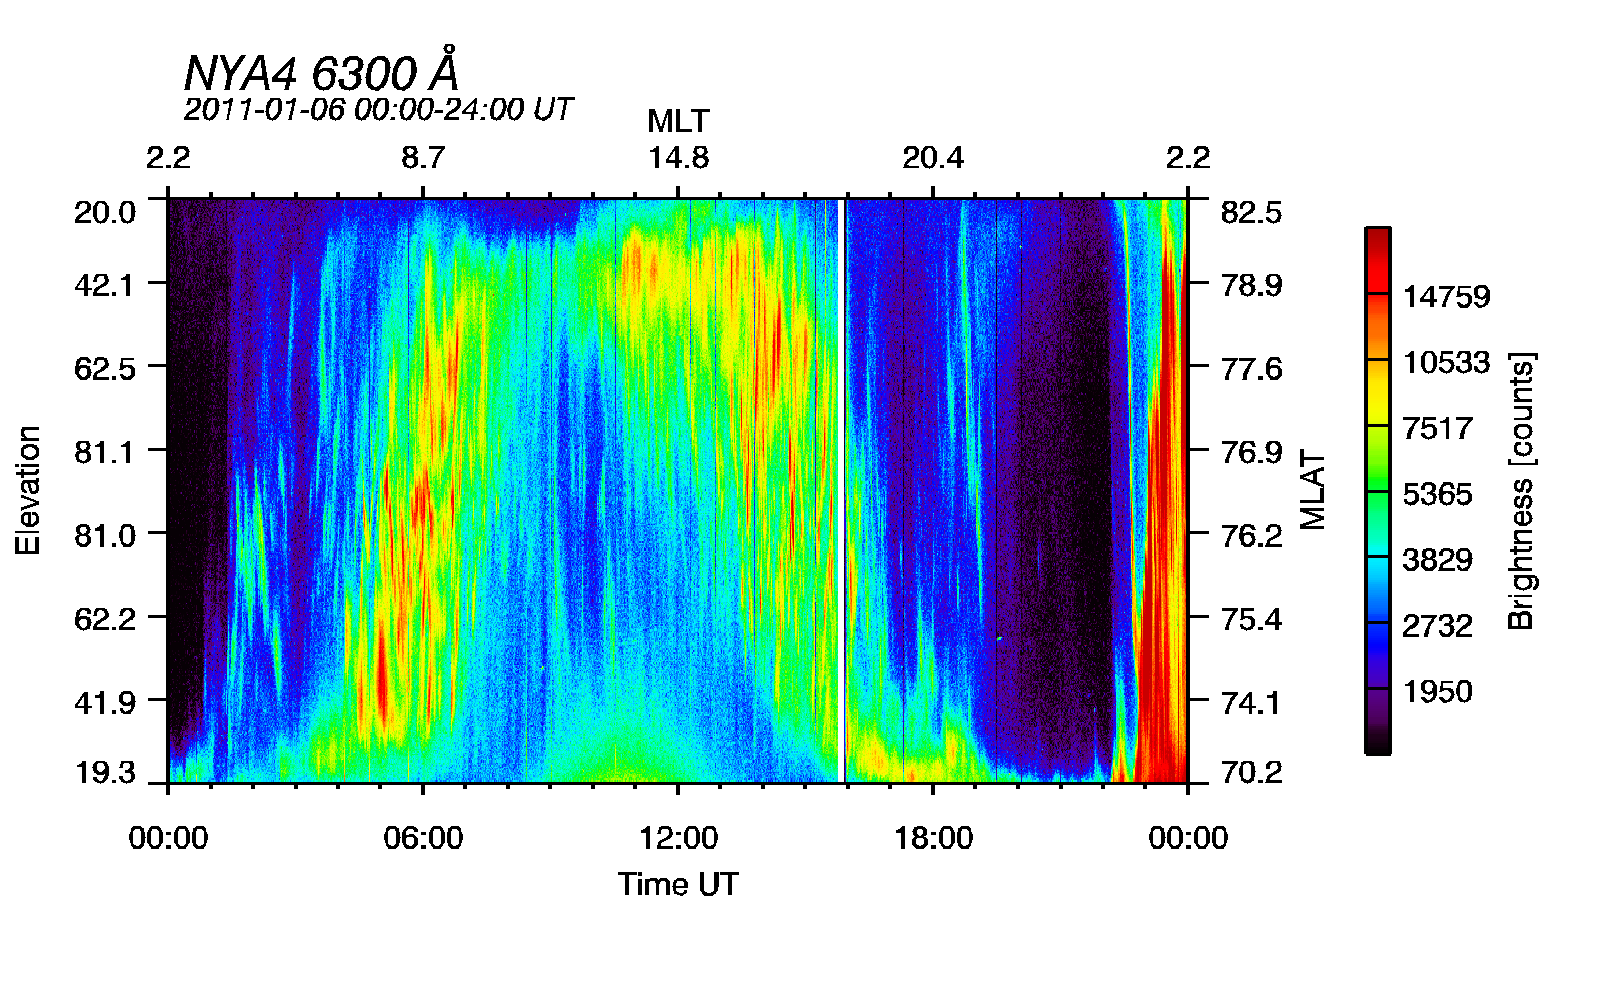
\includegraphics[scale = 0.2]{Figures/nya4_20110106_0000-2400_6300.png}
\centering
\caption{Keograms showing development of aurora over Ny Ålesund the sixth of february 2011. Source: http://tid.uio.no/plasma/aurora/}
\end{figure}
 

\subsection{ACE data} % (All data and observations from ACE)
\label{sub:ACE_data}



\begin{figure}[H]
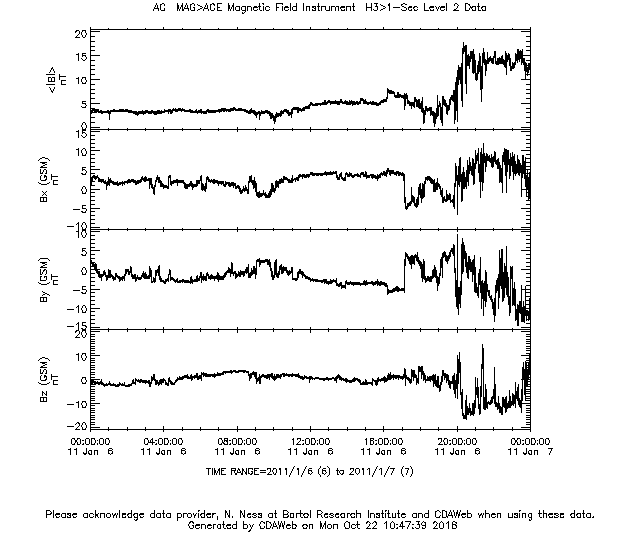
\includegraphics[scale=0.6]{Figures/ACEmagfield2011_01_06.png}
\centering
\caption{Data from the MAG instrument showing the magnetic field in GSM coordinates and the magnitude. Source: \url{http://cdaweb.gsfc.nasa.gov/cdaweb/istp_public/}}
\label{fig:ACEmag}
\end{figure}

\begin{figure}[H]
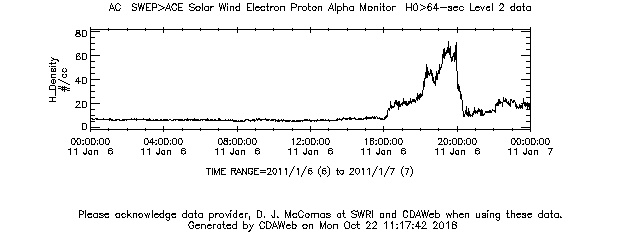
\includegraphics[scale=0.6]{Figures/ACE_H_Density.png}
\centering
\caption{Data from SWEPAM showing the solar wind proton number density. Source: \url{http://cdaweb.gsfc.nasa.gov/cdaweb/istp_public/}}
\label{fig:ACE_H_Density}
\end{figure}

\begin{figure}[H]
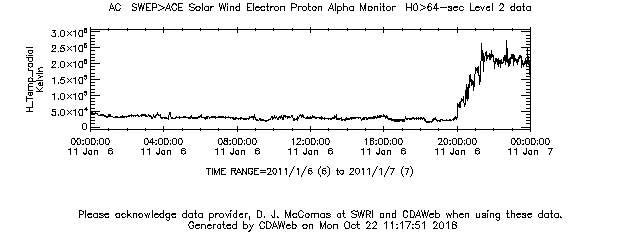
\includegraphics[scale=0.6]{Figures/ACE_H_Temp_radial.png}
\centering
\caption{Data from SWEPAM showing the radial component of the proton temperature. Source: \url{http://cdaweb.gsfc.nasa.gov/cdaweb/istp_public/}}
\label{fig:ACE_temp}
\end{figure}

\begin{figure}[H]
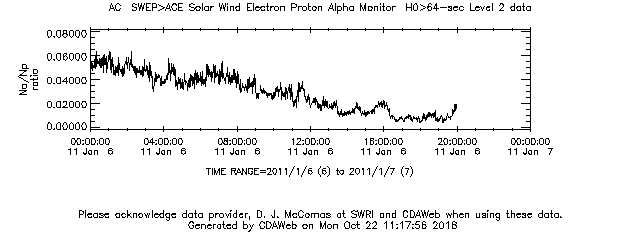
\includegraphics[scale=0.6]{Figures/ACE_Na_Np.png}
\centering
\caption{Data from SWEPAM showing the alpha to proton density ration. Source: \url{http://cdaweb.gsfc.nasa.gov/cdaweb/istp_public/}}
\label{fig:ACE_na_np}
\end{figure}

\begin{figure}[H]
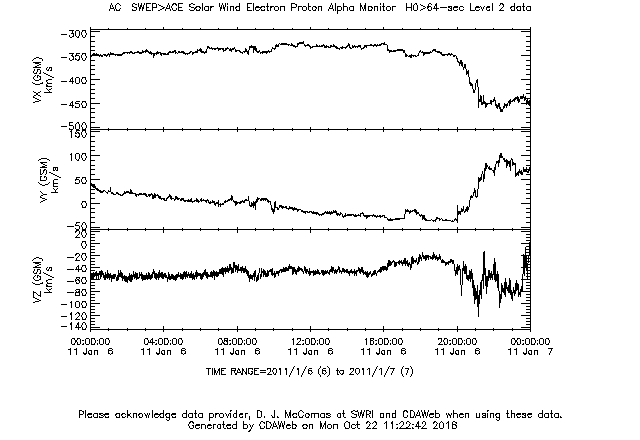
\includegraphics[scale=0.6]{Figures/ACE_SE_velocityGSM.png}
\centering
\caption{Data from SWEPAM showing the solar wind velocity in GSM coordinates. Source: \url{http://cdaweb.gsfc.nasa.gov/cdaweb/istp_public/}}
\label{fig:SWvelGSM}
\end{figure}

\begin{figure}[H]
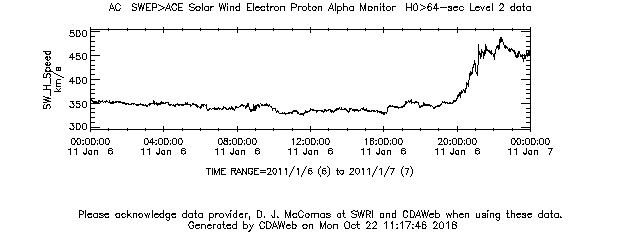
\includegraphics[scale=0.6]{Figures/ACE_SW_H_Speed.png}
\centering
\caption{Data from SWEPAM showing the solar wind bulk speed. Source: \url{http://cdaweb.gsfc.nasa.gov/cdaweb/istp_public/}}
\label{fig:ACE_bulk}
\end{figure}

\begin{figure}[H]
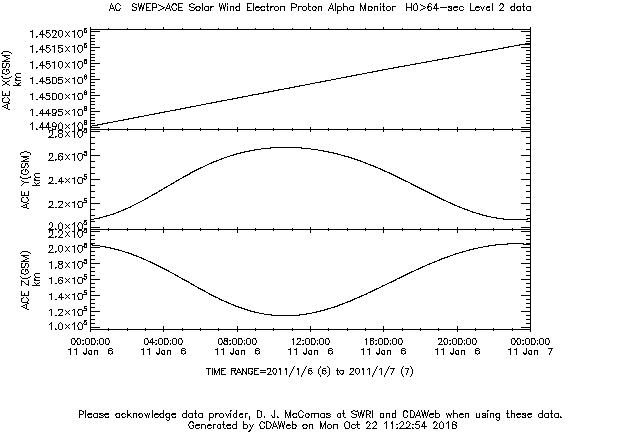
\includegraphics[scale=0.6]{Figures/ACE_positionGSM.png}
\centering
\caption{Data from SWEPAM showing the satellite position in GSM coordinates. Source: \url{http://cdaweb.gsfc.nasa.gov/cdaweb/istp_public/}}
\label{fig:ACE_pos}
\end{figure}

% subsection ace_data (end)


\subsection{Dst data} % (fold)
\label{sub:dst_data}

\begin{figure}[H]
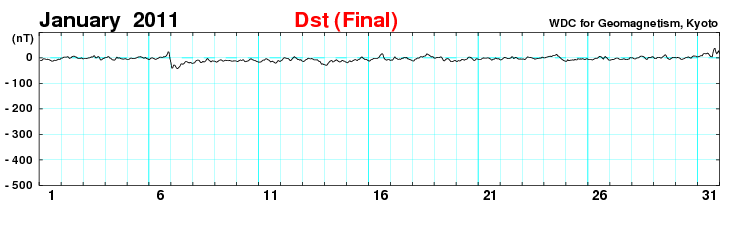
\includegraphics[scale=0.4]{Figures/dst1101.png}
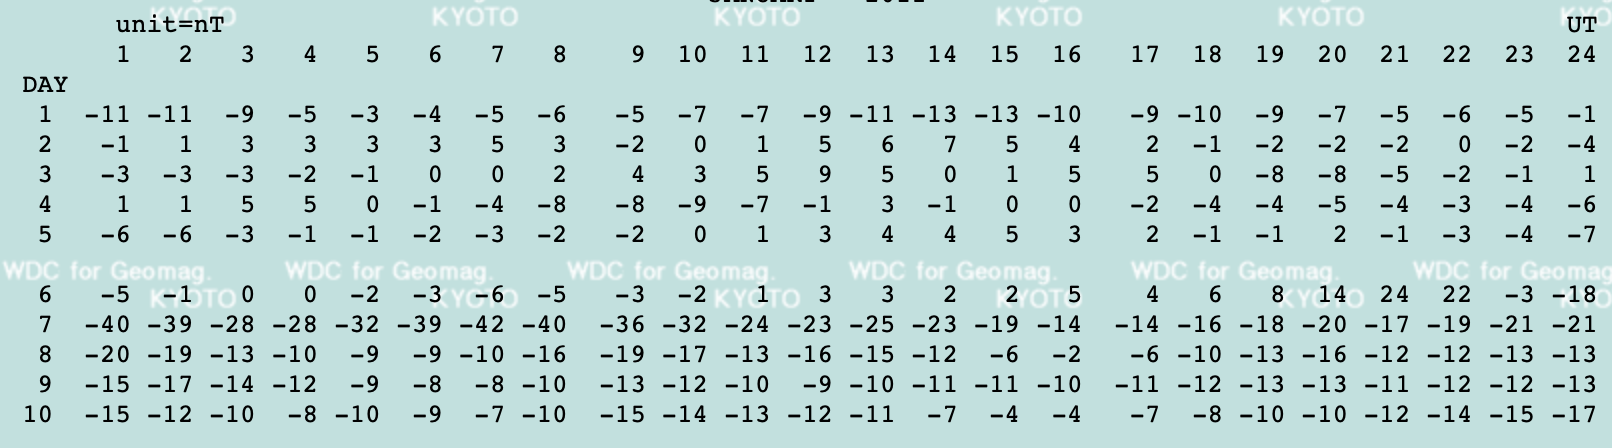
\includegraphics[scale=0.4]{Figures/dst_january.png}
\centering
\caption{The Dst index of January 2011, with values for the 1st to the 10th. source: \url{http://wdc.kugi.kyoto-u.ac.jp/dst_final/201101/index.html}}
\end{figure}

% subsection dst_data (end)

\subsection{AE Index data} % (fold)
\label{sub:AE_index_data}

\begin{figure}[H]
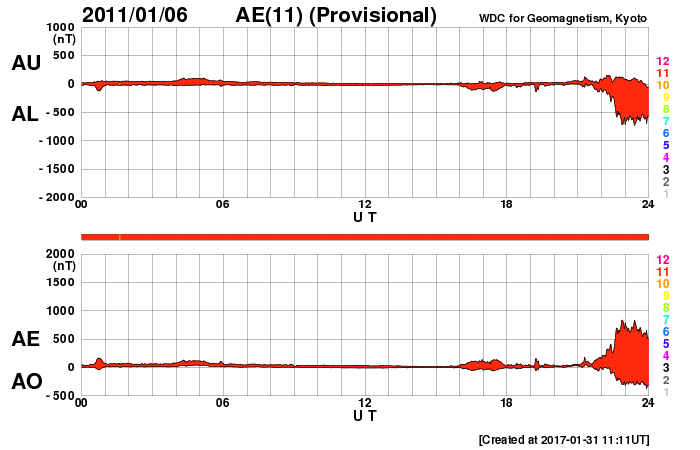
\includegraphics[scale=0.4]{Figures/pvae_2011_01_06.png}
\centering
\caption{The Provisional AE index of January 6. 2011. Source: \url{http://wdc.kugi.kyoto-u.ac.jp/ae_provisional/201101/index_20110106.html}}
\end{figure}

% subsection AE_index_data (end)

\subsection{Kp Index} % (fold)
\label{sub:kp_index}

% subsection kp_index (end)
 
% section observations (end)


\section{Discussion} % (Discussion of the results we got with respect to the observations)
\label{sec:discussion}
First we will begin with analysis of the ACE data. From the MAG instrument, the thing of interest is the IMF Bz componenet of the magnetic field. From midnigt to about 17 the Bz is fluctuating slowly and calmly around 0 nT. After 17 and until 20 the Bz becomes more erratic, with bigger movements. At around 20, there is a sudden jump in Bz up to around 10 nT, after which it plummets to about $- 15 nT$. What follows is a negative Bz almost all the way to midnight, except for a positive spike a little after 21.


% section discussion (end)

\section{Conclusion} % (Conclusion of the discussion and project)
\label{sec:conclusion}

Conclude some shit!
% section conclusion (end)



\section{Appendix} % (fold)
\label{sec:appendix}

% section appendix (end)

\section{Refrences and acknowledgements} % ()
\label{sec:refrences_and_acknowledgements}

% section refrences_and_acknowledgements (end)
\end{document}